% CVPR 2024 Paper Template; see https://github.com/cvpr-org/author-kit

\documentclass[10pt,twocolumn,letterpaper]{article}

\usepackage{cvpr}      % To produce the REVIEW version
% \usepackage[pagenumbers]{cvpr} % To force page numbers, e.g. for an arXiv version

% Import additional packages in the preamble file, before hyperref
%
% --- inline annotations
%
\usepackage[dvipsnames]{xcolor}
\newcommand{\red}[1]{{\color{red}#1}}
\newcommand{\todo}[1]{{\color{red}#1}}
\newcommand{\TODO}[1]{\textbf{\color{red}[TODO: #1]}}
% --- disable by uncommenting  
% \renewcommand{\TODO}[1]{}
% \renewcommand{\todo}[1]{#1}



\definecolor{cvprblue}{rgb}{0.21,0.49,0.74}
\usepackage[pagebackref,breaklinks,colorlinks,citecolor=cvprblue]{hyperref}

\def\paperID{*****} % *** Enter the Paper ID here
\def\confName{CVPR}
\def\confYear{2024}

%%%%%%%%% TITLE - PLEASE UPDATE
\title{Warm Up Assignments}

\author{Rishitosh Kumar Singh\\
Arizona State University\\
% Institution1 address\\
{\tt\small rksing18@asu.edu}
}

\begin{document}
\maketitle


\begin{figure*}[htbp]
    \centering
    \begin{subfigure}{0.2\linewidth}
        \centering
        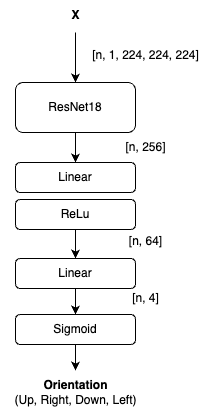
\includegraphics[width=\linewidth]{images/OrientationModel.png}
        \caption{Orientation Model}
        \label{fig:orientation_model}
    \end{subfigure}
    \begin{subfigure}{0.2\linewidth}
        \centering
        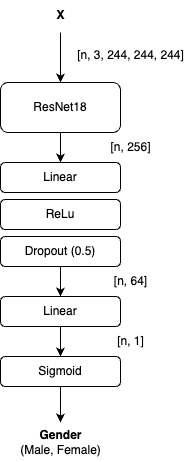
\includegraphics[width=\linewidth]{images/GenderModel.png}
        \caption{Gender Model}
        \label{fig:gender_model}
    \end{subfigure}
    \begin{subfigure}{0.2\linewidth}
        \centering
        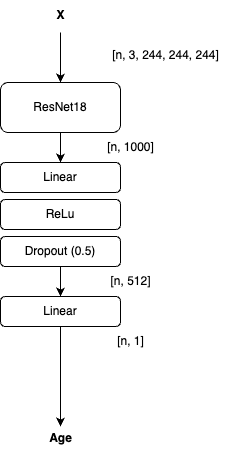
\includegraphics[width=\linewidth]{images/AgeModel.png}
        \caption{Age Model}
        \label{fig:age_model}
    \end{subfigure}
    % \begin{subfigure}{0.5\linewidth}
    %     \centering
    %     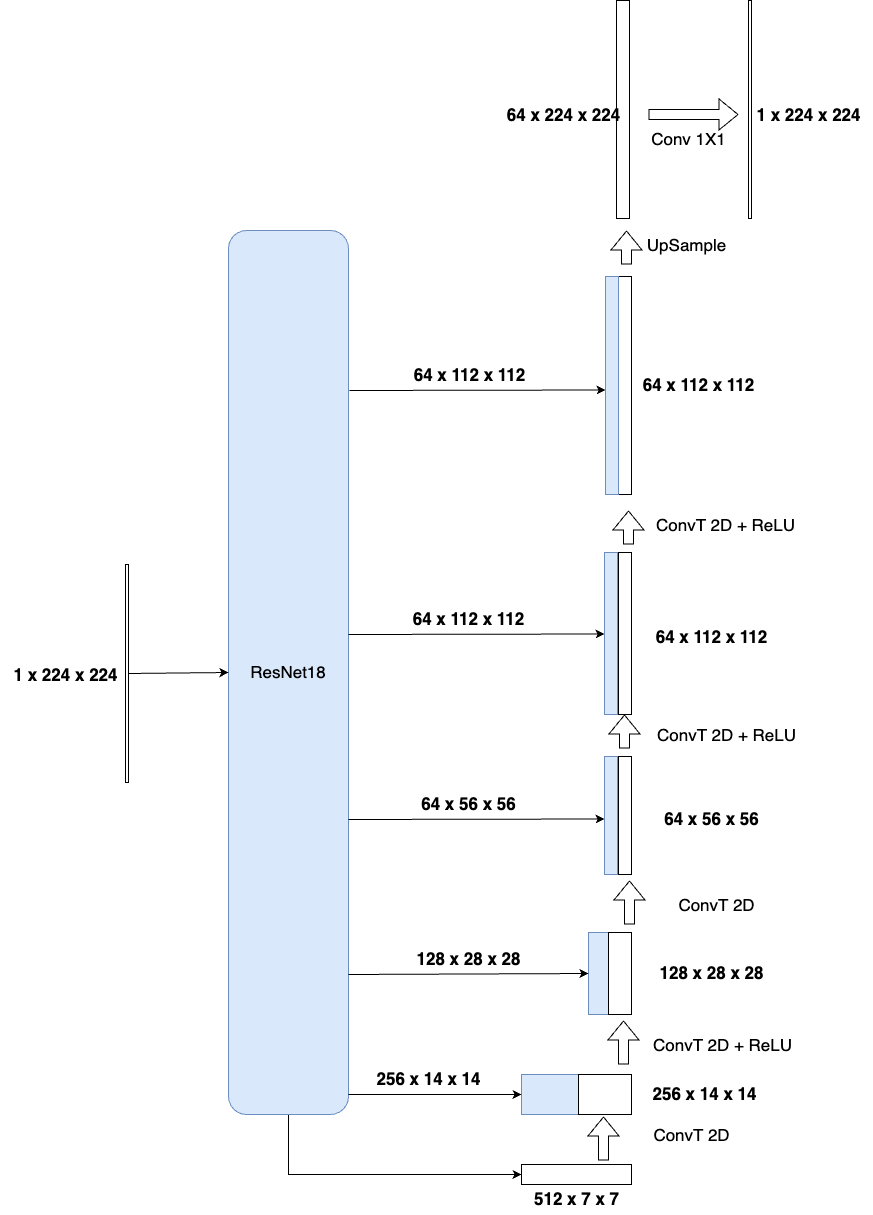
\includegraphics[width=\linewidth]{images/Unet-segmentation.png}
    %     \caption{UNet for lung segmentation}
    %     \label{fig:unet_lung}
    % \end{subfigure}
    
\end{figure*}

\begin{figure}[htbp]
    \centering
    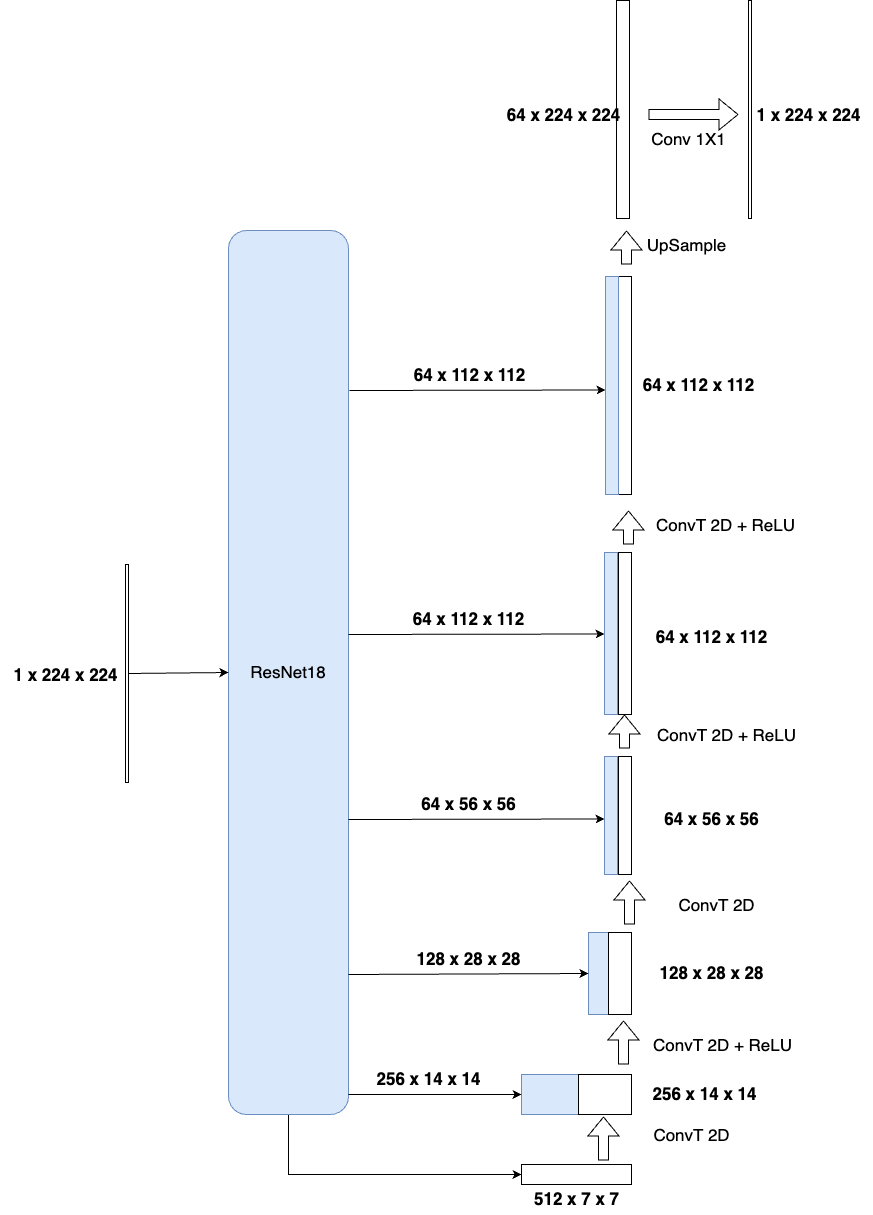
\includegraphics[width=\linewidth]{images/Unet-segmentation.png}
    \caption{UNet for lung segmentation}
    \label{fig:unet_lung}
\end{figure}
\begin{abstract}
    This report is part of the assignment that is due on 21st Jan 2024. This report consists of two practice problems and by completing these problems I got to know how datasets and dataloaders work in Pytorch, and how to train and test a neural network with Pytorch.
\end{abstract}    
\section{Introduction}
\label{sec:intro}
    This report documents the warm-up assignments and will be refined with each subsequent task completion. Additionally, it will incorporate details of new experiments undertaken in each assignment. The overarching goal is to achieve State-of-the-Art (SOTA) performance by employing a diverse array of techniques. A dedicated section labeled "To-Do" will delineate pending tasks for discussion and action. 
    
\section{Backbone models}
    Training a model from scratch consumes substantial resources, including data and time, which may not always be feasible. In scenarios where large datasets are lacking, transfer learning emerges as a practical solution. Transfer learning involves leveraging a pre-trained network with existing weights and fine-tuning it on a new dataset. Typically, backbone models are utilized in the initial layers as they excel at capturing fundamental features. Following these backbone networks, additional layers such as a linear layer or another classifier can be incorporated to adapt to the nuances of the new dataset.

    \subsection{ResNet}
    ResNet, an abbreviation for Residual Network, was pioneered by Kaiming He et al. \cite{he2016deep}. Its hallmark innovation lies in the incorporation of residual connections, a breakthrough technique that remains integral in contemporary state-of-the-art networks, transcending beyond the realm of computer vision tasks. ResNet manifests in various versions, distinguished by the number of layers, including ResNet18, ResNet50, and beyond. Its widespread adoption stems from its capacity to facilitate the utilization of extremely deep networks, a feat made possible by the introduction of residual connections.

    ResNet models are trained on ImageNet dataset, thus it have 1000 output nodes. In order to use it for our problems, we have to append few linear layers after this backbone layer.
\section{Warm Up Exercise 1}
\label{sec:warmup1}
    \subsection{Problem}
        In this exercise, we were provided with two datasets. The objective was to proficiently load the data using PyTorch's dataloaders and dataset APIs, and subsequently, successfully generate matplotlib plots by writing the images.
    \subsection{Solution}
        
    To load the provided dataset, custom PyTorch dataset classes were crafted. These classes offer flexibility to handle datasets of various types and formats. The torchvision.io.read\_image function is employed for reading PNG/JPG images, while the pydicom library is utilized for reading DICOM data.
    
    \subsubsection*{Transformations}
        \begin{figure}[b]
            \begin{subfigure}[t]{\linewidth}
                \centering
                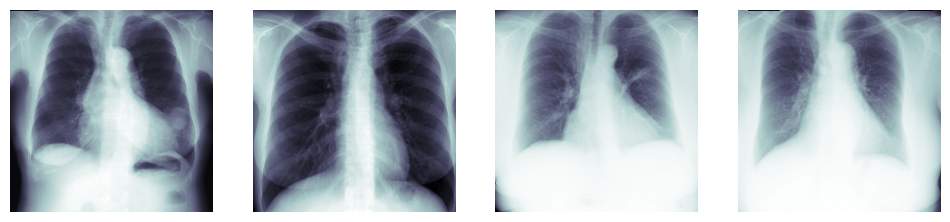
\includegraphics[width=\linewidth]{images/chest-xray-output.png}
                \caption{PNG/JPG dataset}
                \label{fig:png-image}    
            \end{subfigure}
            \begin{subfigure}[t]{\linewidth}
                \centering
                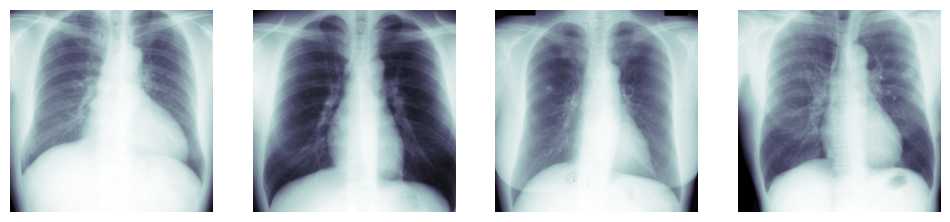
\includegraphics[width=\linewidth]{images/dicom.png}
                \caption{DICOM dataset}
                \label{fig:dicom-image}
            \end{subfigure}
            \caption{XRay images batch}
            \label{fig:xray-images}
        \end{figure}
        \begin{itemize}
            \item When PNG/JPG images were loaded, a resize transformation was applied to change the images to a size of $256$x$256$. \Cref{fig:png-image} displays a batch of 4 images from the PNG/JPG dataset.
            \item After loading DICOM data, a sequence of transformations was employed. At first, the image type is converted from uint16 to uint8, because PyTorch resize function does not support uint16 dtype. Subsequently, the tensor is converted to a PIL image, and the image is resized. Following the dataset loading, all the images are plotted in a matplotlib plot. \Cref{fig:dicom-image} displays a batch of 4 images from the DICOM dataset.
        \end{itemize}
    
\section{Orientation}
\label{sec:warmup2}

    In this introductory practice exercise, chest X-rays were provided, and the task involved training/fine-tuning a model to determine the orientation of these X-rays.

\subsection{Dataset}
    The provided dataset consists of RGB X-ray images with 948 training samples depicting various orientations and an additional 40 samples for testing. All images are of size $128$x$128$ and are oriented either as up (0), right (1), down (2), or left (4). Due to the absence of a dedicated validation set in the given dataset, I have randomly partitioned the training samples into training and validation sets in 8:2 ratio. 
\subsection{Model Used}

    For this task, I utilized ResNet18 as the backbone model with pre-trained weights from ImageNet. Since ResNet18 was originally trained on ImageNet, its output tensor has a size of (n, 1000). However, in the given problem, we are specifically dealing with 4 classes (up, right, down, left). Therefore, I introduced a fully connected layer followed by a log-softmax layer to obtain probabilities for each class. Refer to \Cref{fig:orientation_model} for a graphical representation of the model architecture.
    
    % \begin{figure}[htbp]
    %     \centering
    %     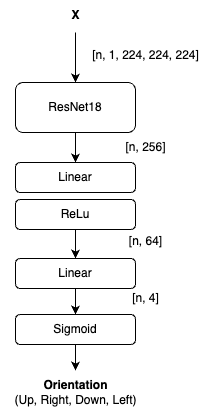
\includegraphics[width=0.4\linewidth]{images/OrientationModel.png}
    %     \caption{Graph of model used}
    %     \label{fig:model_graph}
    % \end{figure}

\subsection{Training}
    
    The model is trained using the categorical cross-entropy loss function with stochastic gradient descent as the optimizer. As the Log-Softmax layer is already included in the model, the torch.nn.NLLLoss function is employed instead of a torch.nn.CrossEntropyLoss. Four experiments were conducted with learning rates of 0.001, 0.003, 0.01, and 0.03, and the results were averaged. Refer to \Cref{fig:learning-curve} for a demonstration of the learning curve from one of the experiments.

    \begin{figure}[htbp]
        \centering
        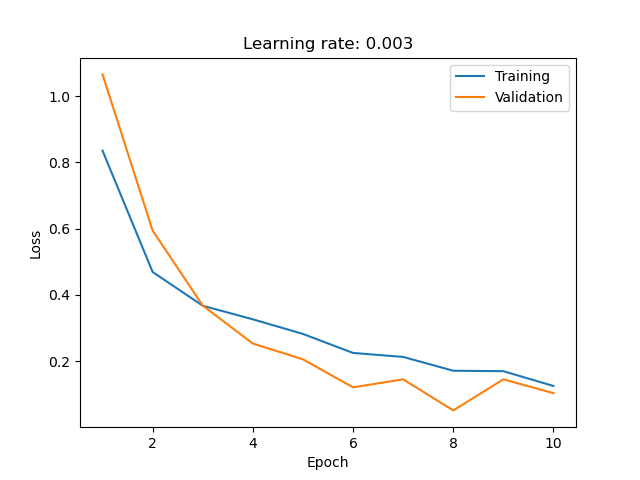
\includegraphics[width=\linewidth]{../plots/orientation/2024-01-20 21:01:42-train-val-plot.png}
        \caption{Learning curve}
        \label{fig:learning-curve}
    \end{figure}

\subsection{Results}

    \begin{figure}[!htbp]
        \centering
        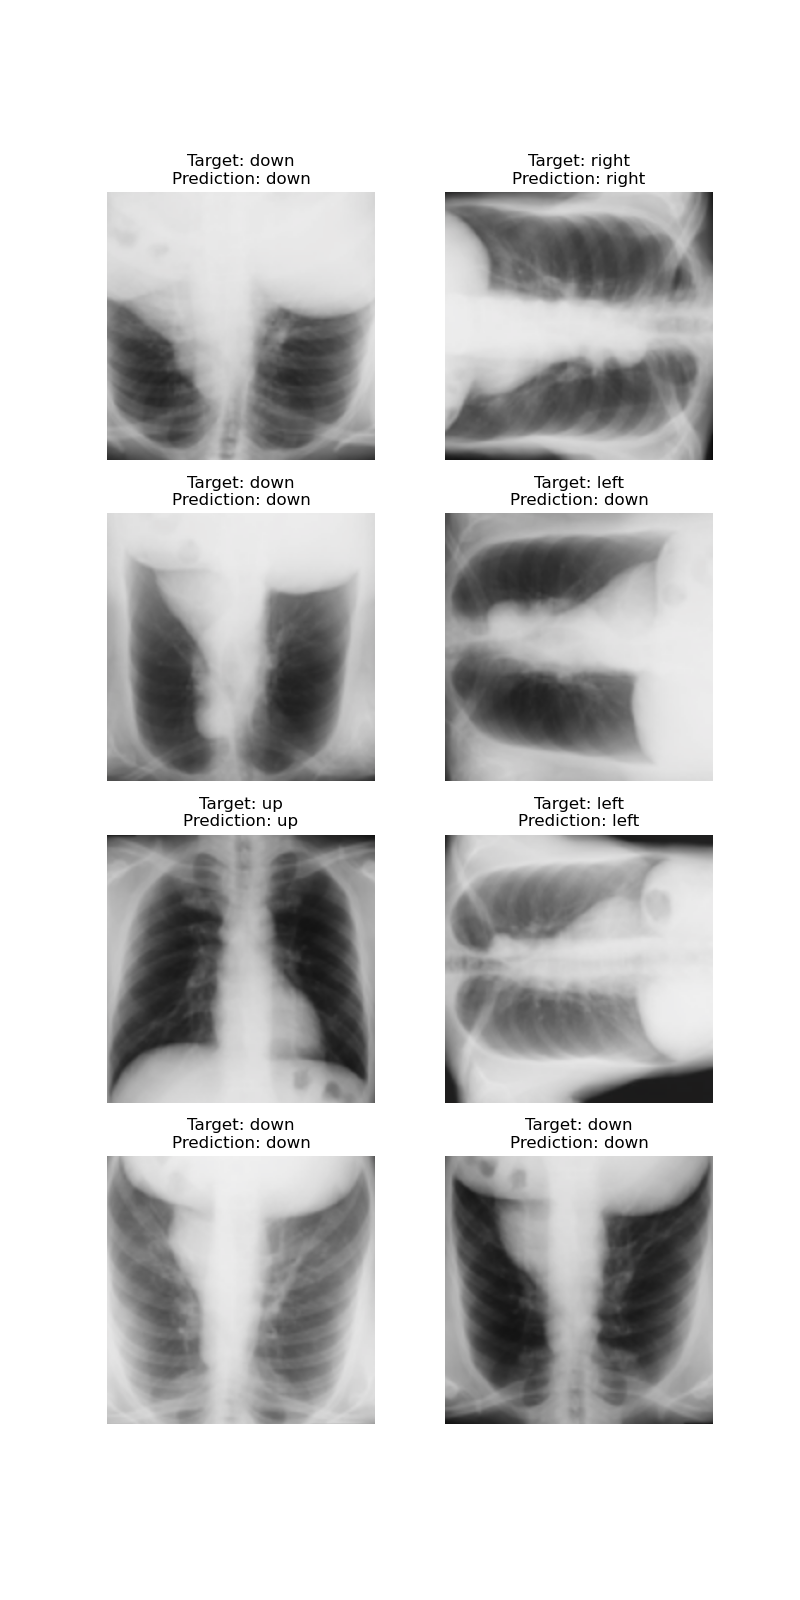
\includegraphics[width=\linewidth]{../plots/orientation/2024-01-20 21:01:42.png}
        \caption{Predictions on few samples of test data}
        \label{fig:results}
    \end{figure} 

    After fine-tuning the model with the ResNet18 backbone network, the model was transitioned to testing and evaluated on the provided test samples. On average, it achieved an accuracy of $96.87\%$, and in some experiments, $100\%$ accuracy was also attained. \Cref{fig:results} showcases some of the test samples along with their model predictions and target classes.

\section{Gender}
\label{sec:warmup3}

    In this preliminary practice activity, we were given chest X-ray images of patients using which we have to either train or fine-tune a model to determine the gender of patients.

\subsection{Dataset}
    We were given three datasets for classifying gender of the patients; grayscale, RGB, and index. Out of these, I have used Gender01\_RGB for the experiments. The provided dataset 154 training samples of patient X-Rays and an additional 93 samples for testing trained model.  The images in this dataset were color image with shape $256$x$256$. Each training samples have either label "male", or "female". Due to the absence of a dedicated validation set in this dataset too, I have randomly partitioned the training samples into training and validation sets in 9:1 ratio.

\subsection{Training}

    In this task, we are dealing with two labels: male and female. Therefore, we constructed a model with a graph described in \cref{fig:gender_model}. A log-softmax layer is employed to obtain probabilities for each class. The model is trained using the categorical cross-entropy loss function with Adam optimizer having a learning rate of $0.003$. We utilize the torch.nn.NLLLoss function, which is commonly used for classification problems, as our loss function. Additionally, early stopping with a patience of 3 epochs is implemented to halt the model training if the validation loss continues to increase for 3 consecutive epochs. \Cref{fig:gender-learning-curve} illustrates the learning curve of the training and validation sets.

    \begin{figure}[htbp]
        \centering
        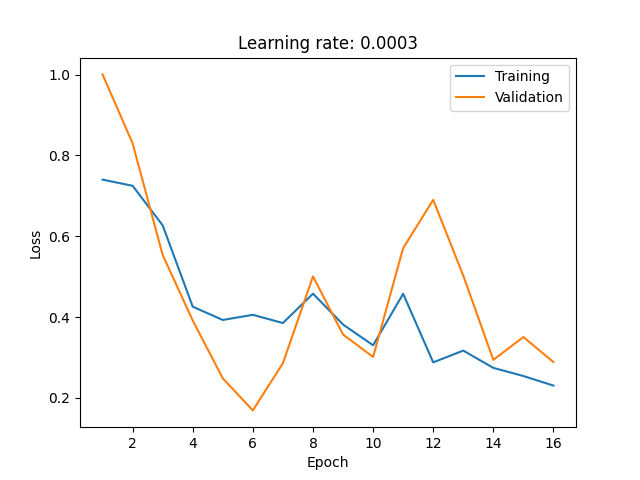
\includegraphics[width=\linewidth]{../outputs/gender/gender1/loss-curve.png}
        \caption{Gender model learning curve on training and validation sets}
        \label{fig:gender-learning-curve}
    \end{figure}

\subsection{Results}

    \begin{figure}[!htbp]
        \centering
        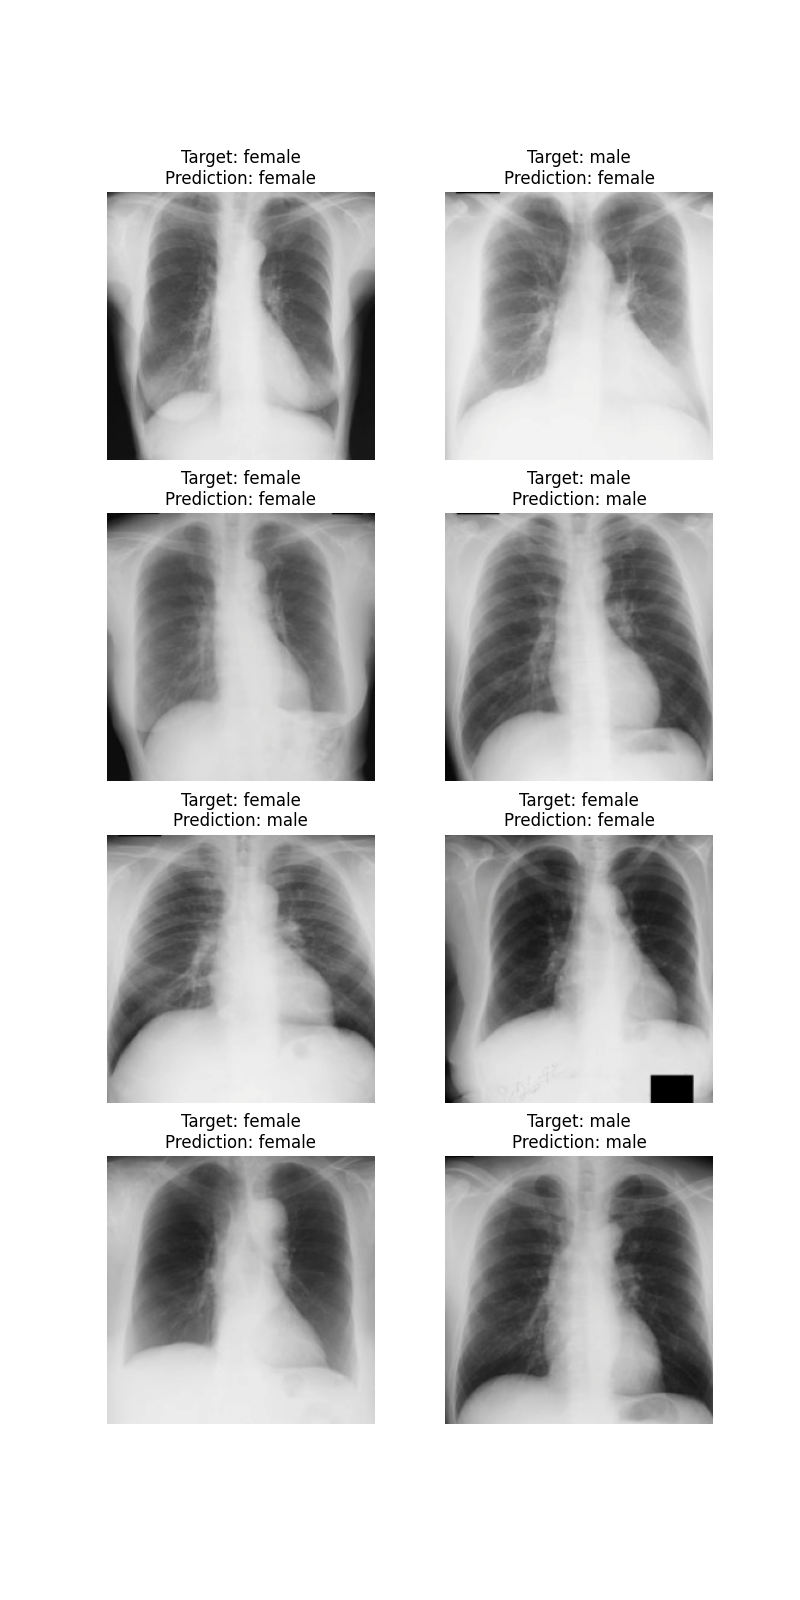
\includegraphics[width=\linewidth]{../outputs/gender/gender1/test-results.png}
        \caption{Gender predictions on few samples of test data}
        \label{fig:gender-results}
    \end{figure} 

    After fine-tuning the model, it was evaluated on the provided test samples on which it achieved an accuracy of $90.32\%$, and AUC of $90.34$. \Cref{fig:gender-results} showcases some of the test samples along with their model predictions and target classes.

\subsection{Find patient age from XRay}
\label{sec:warmup4}

    We were given chest X-ray images of patients using which we have to fine-tune a model to determine the age of patients.

\subsubsection{Dataset}
    The provided dataset have $80$ training x-ray images and $165$ testing images. As there was no validtion set, I have randomly splited the training dataset into validation and training set in ration 1:9 respictively. The images in this dataset were color image with shape $2048 \times 2048$, which is resized to image of size $224 \times 224$.

\subsubsection{Training}

    This is a regression problem, thus a few changes is required to the model used in classifying gender of patients. The last Log Softmax layer is not required, thus eliminated from the model graph as shown in \cref{fig:age_model}. The model is trained using mean ssquare error function with Adam optimizer having a learning rate of $0.003$. Additionally, in this experiment too, early stopping with a patience of 3 epochs is implemented to halt the model training. \Cref{fig:gender-learning-curve} illustrates the learning curve of the training and validation sets.

    \begin{figure}[htbp]
        \centering
        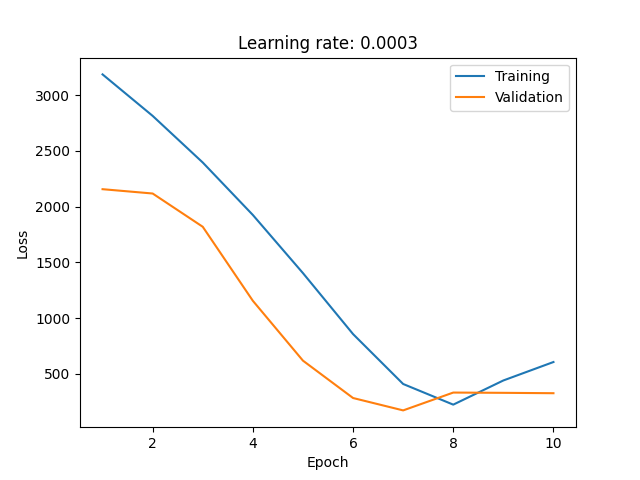
\includegraphics[width=\linewidth]{../outputs/age/age2/loss-curve.png}
        \caption{Age model learning curve on training and validation sets}
        \label{fig:age-learning-curve}
    \end{figure}

\subsubsection{Results}

    \begin{figure}[!htbp]
        \centering
        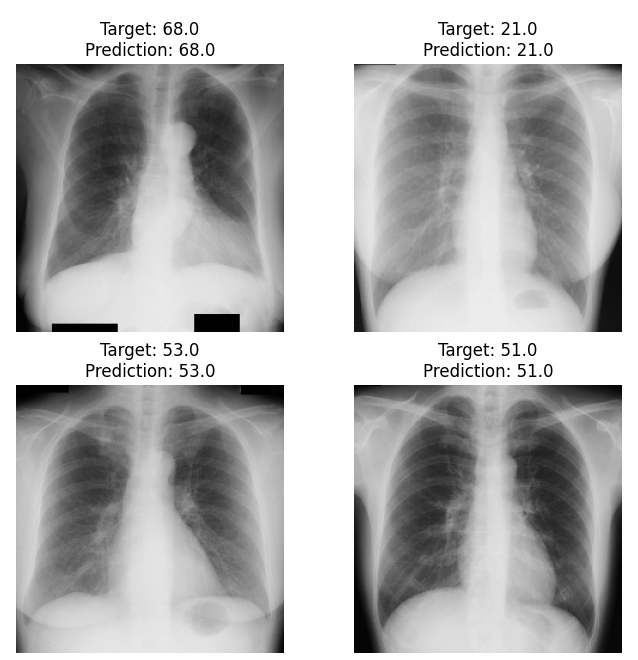
\includegraphics[width=\linewidth]{../outputs/age/age1/test-results-cropped.png}
        \caption{Age predictions on few samples of test data}
        \label{fig:age-results}
    \end{figure} 

    A total of 2 experiments were conducted with same hyperparameters and results are averaged. After fine-tuning the model, it was evaluated on the provided test samples on which it achieved a MAE of $5.57$ \Cref{fig:age-results} showcases some of the test samples along with their model predictions.

\subsection{Segment lungs in XRay(s)}
\label{sec:warmup5}

    Lung segmentation from X-rays are required to automate boundary detection, enhancing diagnostic accuracy and efficiency in medical imaging analysis. In this exercise, we were given chest X-ray images of patients, and the segmented masks of their lungs. We need to employ a deep learning model that can segment lungs from XRays or find boundaries of the lungs.

\subsubsection{Dataset}

    The provided dataset have $50$ training x-ray images and $10$ testing images, with their corresponding masks, thus we can observe that the provided dataset is very small. As there was no validtion set, I have randomly splited the training dataset into validation and training set in ration 1:9 respictively. The images in this dataset were converted to grayscale images with shape $256 \times 256$.

\subsubsection{Training}

    This being a segmentation problem, an encoder-decoder type of model needs to be employed. I have created a UNet as shown in \cref{fig:unet_lung}. The model have a resnet18 encoder block which was pretrained on imagenet1k dataset and a decoder block. As the model might suffers from gradient vanishing, skip connections is used, thus a UNet is structure is achieved. Since, I am predicting the pixels of an image as $0$ or $1$, binary cross-entropy error was used for training with Adam optimizer with learning rate of $10^{-3}$. \Cref{fig:lung-segmentation-learning-curve} illustrates the learning curve of the training and validation sets.

    \begin{figure}[htbp]
        \centering
        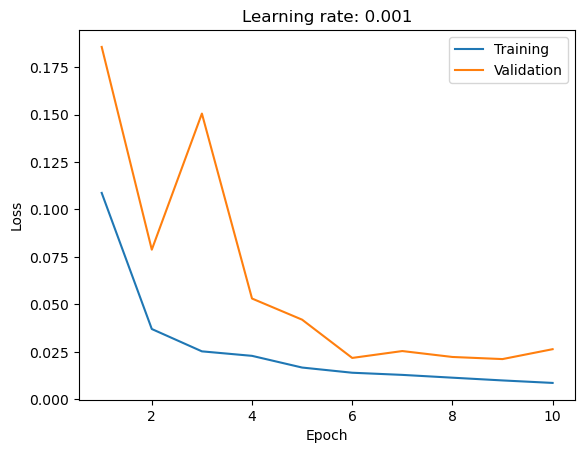
\includegraphics[width=\linewidth]{../plots/segmentation/learning.png}
        \caption{Lungs segmentation model learning curve on training and validation sets}
        \label{fig:lung-segmentation-learning-curve}
    \end{figure}

\subsubsection{Results}

    From the learning curve in \cref{fig:lung-segmentation-learning-curve} we can observe that the model have converged to lowest loss, and is not overfited on the dataset. The trained model is then tested on test set, and got mIoU score of $0.933$ and mDICE score of $0.965$. \Cref{fig:lung-segmentation-result} shows the predicted lung mask of a XRay and we can observe that model is able to generate masks which is similar to ground truth mask.

    \begin{figure}[htbp]
        \centering
        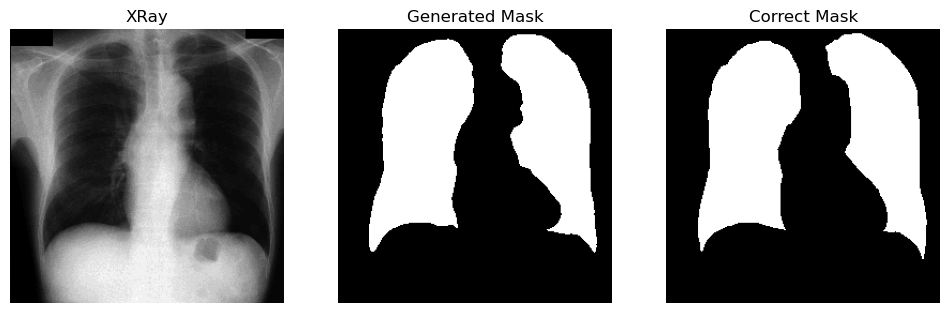
\includegraphics[width=\linewidth]{../plots/segmentation/result.png}
        \caption{Predicted lung mask of an XRay by trained UNet}
        \label{fig:lung-segmentation-result}
    \end{figure}
\section{Multiple Segmentation}
\label{sec:warmup6}

    We were given chest X-ray images of patients and corresponding mask image. The mask image have a total of $4$ masks; lungs, heart, body, and background. Our task is to create a model and train it to generate these segmentation masks.

\subsection{Dataset}
    The provided dataset have $200$ training x-ray images and $47$ testing images. As there was no validtion set, I have randomly splited the training dataset into validation and training set in ration 1:9 respictively. Validation set is important as it allows one to verify model performance on hold-out set.

\subsection{Training}

    This problem and the previous problems are similar in a way the only difference is that in this problem there are 4 masks instead of one. The same model (\cref{fig:unet_lung}) after modifying the last layer can be utilized for this task. The output channel needs to be changed from $1$ to $4$. 
    
    The dataset also needs to be modified. The label images, which are grayscale images, needs to be changed to 4 channel images, in which each channel have only one mask. 

    The task is incomplete as expected result was not received in last proble,
\section{To-Do}

\begin{itemize}
    \item Use anomalib with trained model to find anamolies in chest xrays. 
    \item Improve report by paraphrasing.
    \item Include Conclusion
\end{itemize}
{
    \small
    \bibliographystyle{ieeenat_fullname}
    \bibliography{main}
}

% WARNING: do not forget to delete the supplementary pages from your submission 
% \input{sec/X_suppl}

\end{document}
